\chapter{Proiectare de detaliu și implementare}
\pagestyle{fancy}
\setlength{\parskip}{0.35em}
\setlength{\intextsep}{10pt plus 2pt minus 2pt}
\setlength{\textfloatsep}{10pt plus 2pt minus 2pt}

Capitolul de față descrie modul în care soluția propusă a fost proiectată și implementată, pornind de la arhitectura generală și coborând treptat spre componentele concrete ale aplicației. După prezentarea imaginii de ansamblu, capitolul detaliază clientul desktop, modelul intern de adnotare, mecanismele de salvare și export, integrarea worker-elor pentru modele AI, serviciile backend, comunicarea în timp real, persistența datelor și infrastructura de rulare. Scopul capitolului nu este reluarea elementelor teoretice din analiza anterioară, ci explicarea deciziilor de proiectare care leagă modulele implementate într-un sistem funcțional.

\section{Arhitectura generală a sistemului}

Sistemul este organizat în jurul unei aplicații desktop de adnotare, care comunică atât cu modele locale de inteligență artificială, cât și cu un backend împărțit în servicii specializate. La nivel conceptual, aplicația poate fi privită ca o combinație între o zonă interactivă, folosită direct de utilizator pentru încărcarea imaginilor și editarea adnotărilor, o zonă de procesare automată, responsabilă de operațiile AI, și o zonă de servicii, responsabilă de autentificare, chat, colaborare și sincronizare.

\begin{figure}[H]
    \centering
    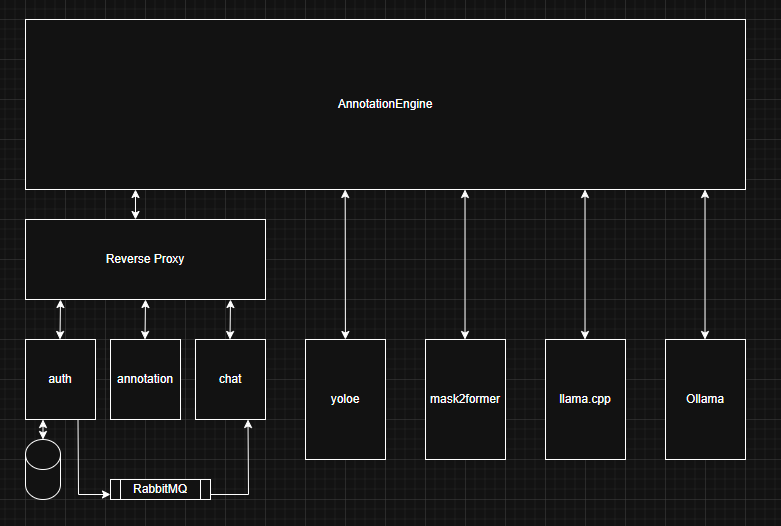
\includegraphics[width=\textwidth]{figs/overview-of-the-project.png}
    \caption{Arhitectura generală a aplicației}
    \label{fig:arhitectura-generala-aplicatie}
\end{figure}

Figura~\ref{fig:arhitectura-generala-aplicatie} prezintă legătura dintre componentele principale ale proiectului. În partea de client se află modulul \texttt{AnnotationEngine}, aplicația desktop scrisă în Python cu PyQt6. Acesta concentrează interacțiunea utilizatorului cu imaginile, uneltele de desenare, lista de etichete, mecanismele de import/export și ferestrele auxiliare pentru autentificare, chat și chatbot local. Din perspectiva utilizatorului, clientul desktop este punctul central al sistemului, deoarece toate acțiunile pornesc din interfața grafică.

A doua zonă importantă este \texttt{ColaborativeServer}, care grupează serviciile backend dezvoltate cu Spring Boot. Backend-ul nu este implementat ca o singură aplicație monolitică, ci ca un set de servicii cu responsabilități separate: serviciul de autentificare gestionează utilizatorii și token-urile JWT, serviciul de chat gestionează conversațiile și prezența, iar serviciul de annotation gestionează sesiunile colaborative și starea comună a adnotărilor. Această separare face ca funcțiile aplicației să poată evolua independent și reduce dependența dintre autentificare, comunicare și sincronizarea efectivă a lucrului pe imagini.

A treia zonă este reprezentată de directorul \texttt{research}, folosit pentru experimentare, testare și comparație între modele sau variante de integrare. Această parte nu este interfața principală a utilizatorului final, dar are rol practic în proiect: aici pot fi testate modele precum YOLOE sau Mask2Former, pot fi verificate intrări și ieșiri, iar rezultatele stabile pot fi apoi integrate în fluxurile controlate de aplicația desktop. Separarea zonei de cercetare de codul clientului ajută la păstrarea aplicației mai curate și permite modificarea experimentelor fără a afecta direct interfața utilizatorului.

O decizie importantă de proiectare este separarea dintre client, modelele externe și backend. Clientul desktop trebuie să rămână responsiv, deoarece utilizatorul poate lucra cu imagini, măști și forme geometrice care necesită randare și interacțiune directă. Modelele AI pot avea timpi de execuție mai mari, pot depinde de biblioteci specializate și pot necesita procese separate. Din acest motiv, ele nu sunt apelate direct în firul principal al interfeței, ci prin worker-e sau procese externe. În acest mod, operații precum segmentarea automată, generarea de măști sau conversația cu un LLM local pot rula fără a bloca aplicația.

Pentru zona de adnotare automată, clientul folosește worker-e dedicate care pornesc sau comunică cu executabile și scripturi externe. AutoSeg este responsabil pentru detecție și segmentare automată pe baza unui model YOLO, în timp ce AutoMask folosește un model de segmentare pe mască pentru a produce contururi mai precise în jurul obiectelor. Rezultatele acestor procese sunt transformate în structuri compatibile cu modelul intern de adnotare al aplicației, astfel încât utilizatorul să le poată corecta, redenumi sau exporta la fel ca pe adnotările create manual.

Un principiu similar este folosit și pentru integrarea modelelor conversaționale locale. Aplicația nu depinde de un serviciu cloud pentru chatbot, ci poate folosi local \texttt{llama.cpp} prin \texttt{llama-cpp-python} sau Ollama prin clientul său local. În arhitectură, aceste modele sunt tratate ca servicii locale auxiliare: interfața trimite mesajele către worker, worker-ul gestionează apelul către motorul LLM, iar răspunsul este readus în aplicație sub formă de mesaj afișabil. Această abordare păstrează controlul asupra resurselor locale și face posibilă rularea funcțiilor AI chiar și în scenarii în care conectivitatea externă nu este o condiție de bază.

Backend-ul completează funcțiile locale prin mecanisme de colaborare și sincronizare. Autentificarea este expusă prin endpoint-uri HTTP/REST, iar sesiunile de lucru și schimbul de evenimente sunt gestionate prin WebSocket și STOMP. În practică, clientul se autentifică, primește un token JWT, apoi îl folosește pentru a accesa funcțiile care necesită identitatea utilizatorului. Pentru operațiile în timp real, evenimentele nu sunt trimise ca cereri izolate, ci ca mesaje publicate către canale asociate sesiunilor, ceea ce permite mai multor clienți să vadă modificări și mesaje pe măsură ce acestea apar.

Infrastructura de rulare este definită cu Docker, astfel încât serviciile backend și dependențele lor să poată fi pornite într-un mod controlat. În configurația proiectului, Traefik are rol de reverse proxy și direcționează cererile către serviciile corespunzătoare. RabbitMQ este folosit ca broker AMQP pentru evenimente între servicii, de exemplu pentru propagarea unor informații despre utilizatori între modulul de autentificare și celelalte module. Pentru datele persistente ale autentificării se folosește Postgres, iar componentele de chat și colaborare păstrează o parte din stare în memorie, deoarece natura lor este mai apropiată de sesiuni active și evenimente de lucru.

Această arhitectură susține două moduri de lucru care apar frecvent în aplicație. În modul individual, utilizatorul poate încărca imagini, crea adnotări manuale, apela modele AI locale și exporta rezultatele fără a depinde de colaborarea cu alți utilizatori. În modul colaborativ, aceleași acțiuni sunt completate de autentificare, camere de lucru, mesaje și sincronizare prin backend. Din acest motiv, clientul desktop este proiectat ca un punct de coordonare: el poate lucra local cu fișiere și worker-e, dar poate folosi și serviciile backend atunci când este necesară partajarea stării între mai mulți utilizatori.

Prin această împărțire, proiectul rămâne modular. \texttt{AnnotationEngine} se concentrează pe experiența de adnotare și pe integrarea locală a modelelor, \texttt{ColaborativeServer} gestionează identitatea și comunicarea între utilizatori, iar zona \texttt{research} permite evoluția componentelor AI fără a destabiliza aplicația principală. În secțiunile următoare, fiecare dintre aceste zone este detaliată din perspectiva implementării: structura clientului, reprezentarea adnotărilor, worker-ele AI, fluxurile de comunicare și serviciile backend care susțin colaborarea.

\section{Structura clientului desktop PyQt}

Clientul desktop reprezintă partea aplicației cu care utilizatorul lucrează direct. În proiect, această componentă este implementată în directorul \texttt{AnnotationEngine} și are rolul de a transforma funcționalitățile sistemului într-un flux de lucru vizual: deschiderea unui set de imagini, desenarea adnotărilor, ajustarea proprietăților, apelarea modelelor externe, exportul datasetului și conectarea la funcțiile colaborative. Spre deosebire de backend, care este împărțit în servicii, clientul desktop este o aplicație interactivă, în care timpul de răspuns al interfeței și claritatea acțiunilor sunt importante pentru utilizator.

\subsection{Rolul clientului desktop în sistem}

Aplicația pornește din fișierul \texttt{app.py}. Acesta creează obiectul \texttt{QApplication}, setează numele aplicației, aplică stilul vizual de bază și deschide fereastra principală \texttt{MainWindow}. Tot aici există și o etapă de inițializare pentru backend-urile AI care pot fi livrate împreună cu aplicația. Funcția de inițializare caută în directoare precum \texttt{inference\_backends}, \texttt{dist} sau \texttt{models} executabile pentru AutoMask, executabile YOLO și fișiere de ponderi \texttt{.pt}, apoi completează valorile lipsă în \texttt{QSettings}. Astfel, aplicația poate porni cu o configurare inițială utilă, fără ca utilizatorul să introducă manual toate căile atunci când executabilele se află deja lângă program.

Din punct de vedere funcțional, \texttt{AnnotationEngine} poate fi folosit în două moduri. Primul este modul local, în care utilizatorul încarcă imagini dintr-un folder, creează adnotări manuale sau automate și exportă rezultatele în formate potrivite pentru antrenarea sau testarea unor modele. Al doilea este modul conectat, în care aplicația folosește autentificarea, chatul și colaborarea în timp real. Această dublă natură explică de ce în client există atât componente de interfață pur locale, precum canvasul și panourile de editare, cât și componente care comunică prin HTTP sau WebSocket cu serviciile din \texttt{ColaborativeServer}.

\begin{figure}[H]
    \centering
    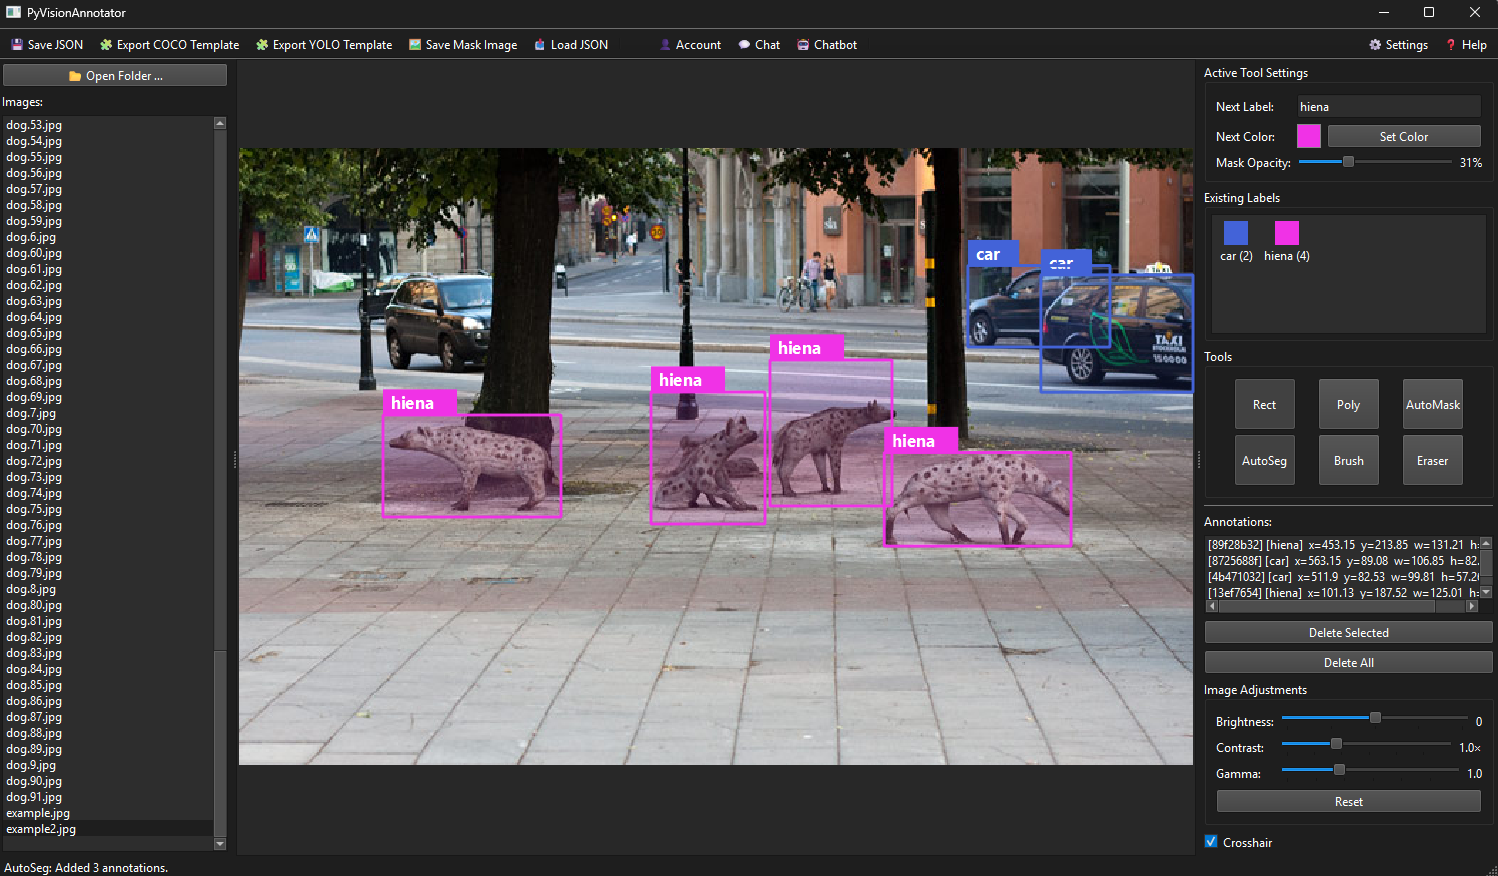
\includegraphics[width=\textwidth]{figs/PyVisionAnnotator.png}
    \caption{Interfața principală a aplicației PyVisionAnnotator}
    \label{fig:pyvisionannotator-interfata-principala}
\end{figure}

După cum se observă în Figura~\ref{fig:pyvisionannotator-interfata-principala}, interfața este împărțită în zone care urmăresc fluxul natural de lucru al utilizatorului. În partea stângă se află lista de imagini din folderul curent, zona centrală este canvasul pe care se afișează imaginea și adnotările, iar panoul din dreapta conține proprietățile obiectului selectat, uneltele active și lista de adnotări. Această împărțire permite utilizatorului să navigheze rapid între imagini, să lucreze direct pe conținutul vizual și să modifice etichetele, culorile sau setările fără a părăsi fereastra principală.

Clientul desktop nu integrează modelele AI direct în codul UI. AutoSeg, AutoMask, Ollama și llama.cpp sunt tratate ca servicii locale sau procese externe, apelate prin worker-e. Această decizie păstrează interfața mai stabilă și reduce dependența dintre codul de desenare și bibliotecile de inferență. Dacă un model este schimbat, ambalat într-un executabil nou sau rulat cu alte argumente, fluxul general al aplicației rămâne același: UI-ul colectează parametrii, worker-ul execută operația, rezultatul este convertit în adnotări.

\subsection{\texttt{MainWindow} ca orchestrator al aplicației}

Clasa \texttt{MainWindow}, definită în \texttt{ui/main\_window/main\_window.py}, este centrul de coordonare al clientului desktop. Rolul ei nu este să implementeze toate detaliile fiecărei funcții, ci să construiască interfața, să conecteze semnalele dintre componente și să păstreze starea comună necesară pentru fluxurile care traversează mai multe module. Din acest motiv, fereastra principală conține referințe către managerul de adnotări, canvas, panouri, worker-ele active și ferestrele auxiliare pentru chat sau chatbot.

Construirea interfeței este concentrată în metoda \texttt{\_build\_ui()}. În această metodă se creează \texttt{AnnotationCanvas}, \texttt{LeftPanel}, \texttt{RightPanel} și \texttt{ToolbarPanel}. Cele trei zone principale ale ferestrei sunt așezate într-un \texttt{QSplitter} orizontal, cu panoul de imagini în stânga, canvasul în centru și panoul de proprietăți în dreapta. Canvasul primește factorul de întindere cel mai mare, deoarece el este zona de lucru efectivă, în timp ce panourile laterale sunt zone de control și navigare.

Metoda \texttt{\_connect\_signals()} definește fluxul reactiv al aplicației. Panourile nu modifică direct toate celelalte componente, ci emit semnale care sunt conectate la metode din \texttt{MainWindow}, \texttt{AnnotationCanvas} sau \texttt{AnnotationManager}. Această separare este importantă pentru întreținere: un buton din panoul drept nu are nevoie să cunoască detaliile de încărcare a imaginilor sau de colaborare, ci doar să emită o intenție, de exemplu schimbarea uneltei active. Fereastra principală decide apoi unde ajunge acea intenție.

\begin{verbatim}
self._left.image_load_requested.connect(self._on_image_load_requested)
self._right.tool_changed.connect(self._canvas.set_tool)
self._canvas.image_loaded.connect(self._on_image_loaded)
self._manager.annotation_added.connect(self._on_data_changed)
\end{verbatim}

Fragmentul de mai sus ilustrează stilul de comunicare folosit în aplicație. Panoul stâng cere încărcarea unei imagini, panoul drept schimbă unealta activă a canvasului, canvasul anunță că imaginea a fost încărcată, iar managerul anunță că datele s-au modificat. În locul unui flux liniar rigid, aplicația folosește semnale și sloturi pentru a păstra componentele decuplate. Acest model este potrivit pentru aplicația de adnotare, deoarece multe acțiuni pot porni din interfață: click în canvas, selecție în listă, buton din toolbar, răspuns de la worker sau eveniment primit din colaborare.

A treia metodă relevantă este \texttt{\_setup\_shortcuts()}, care definește scurtături pentru acțiunile frecvente. \texttt{Delete} șterge adnotarea selectată, \texttt{Ctrl+O} deschide un folder de imagini, iar \texttt{Ctrl+S} salvează adnotările în format JSON. Deși sunt detalii mici, aceste scurtături arată că aplicația este gândită ca instrument de lucru repetitiv, nu doar ca prototip demonstrativ.

\begin{figure}[H]
    \centering
    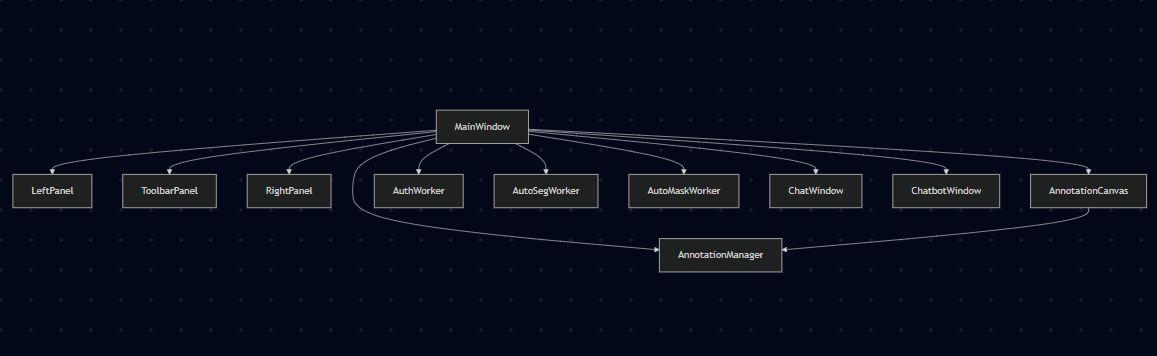
\includegraphics[width=\textwidth]{figs/flowchart_MainWindow.png}
    \caption{Organizarea internă a ferestrei principale}
    \label{fig:organizare-mainwindow}
\end{figure}

Figura~\ref{fig:organizare-mainwindow} trebuie să evidențieze faptul că \texttt{MainWindow} nu este doar o fereastră grafică, ci un strat de orchestrare. În această clasă se păstrează stări precum \texttt{\_unsaved\_changes}, \texttt{\_ignore\_changes}, \texttt{\_applying\_remote\_collab}, referințele către worker-ele active și referințele către ferestrele auxiliare. Aceste stări nu aparțin unui singur panou, deoarece influențează mai multe părți ale aplicației: salvarea, încărcarea, colaborarea, închiderea aplicației și prevenirea trimiterii unor evenimente duplicate.

Pentru a evita transformarea clasei principale într-un fișier foarte greu de urmărit, o parte din fluxuri este extrasă în module din \texttt{utils/main\_window\_parts}. De exemplu, încărcarea imaginilor este tratată în \texttt{load\_process.py}, starea de modificări nesalvate în \texttt{dirty\_state.py}, autentificarea în \texttt{auth\_handlers.py}, iar integrarea AutoSeg și AutoMask în fișiere dedicate. Această împărțire păstrează \texttt{MainWindow} ca punct de conectare, dar mută detaliile operaționale în module tematice.

\subsection{Panourile aplicației}

Interfața principală este împărțită în trei panouri și o bară de unelte. Fiecare panou are o responsabilitate clară, iar comunicarea cu restul aplicației se face prin semnale. Această structură reduce dependențele circulare și permite modificarea unui panou fără rescrierea întregii ferestre principale.

\texttt{LeftPanel} este panoul de navigare prin imagini. El permite deschiderea unui folder, filtrează fișierele după extensii de imagine precum \texttt{jpg}, \texttt{png}, \texttt{bmp}, \texttt{tiff} sau \texttt{webp} și afișează rezultatul într-o listă. Atunci când utilizatorul selectează o imagine, panoul emite \texttt{image\_load\_requested}. O funcție importantă a acestui panou este protecția la schimbarea imaginii atunci când există adnotări nesalvate. În această situație, utilizatorul poate salva, poate continua fără salvare sau poate anula schimbarea. Panoul nu face salvarea direct, ci cere ferestrei principale să o realizeze, deoarece toolbar-ul și managerul de adnotări dețin datele necesare.

\texttt{ToolbarPanel} concentrează acțiunile globale ale aplicației. De aici se pot salva adnotările în JSON, exporta datele în template COCO sau YOLO, salva o imagine cu măștile desenate, încărca un fișier JSON, deschide dialogul de cont, fereastra de chat, fereastra de chatbot și dialogul de setări. Toolbar-ul deține și logica de export, deoarece exportul este o acțiune globală asupra imaginii curente și asupra tuturor adnotărilor din \texttt{AnnotationManager}.

\texttt{SettingsDialog}, deschis din toolbar, este organizat pe taburi. Un tab controlează stilul vizual al adnotărilor, cum ar fi grosimea conturului, dimensiunea fontului și înălțimea etichetei. Alt tab configurează AutoMask, prin calea către executabil, timeout, device și argumente suplimentare. Un tab separat configurează AutoSeg YOLO, prin executabil, fișierul de ponderi, pragul de confidență, device și argumente custom. Ultimul tab gestionează endpoint-urile pentru autentificare. Faptul că aceste valori sunt păstrate în \texttt{QSettings} permite aplicației să rețină configurarea între rulări.

\begin{figure}[H]
    \centering
    
\includegraphics[width=\textwidth]{figs/settings_app.png}
    \caption{Panoul de setări pentru AutoSeg și AutoMask}
    \label{fig:setari-autoseg-automask}
\end{figure}

\texttt{RightPanel} este panoul în care utilizatorul controlează adnotarea curentă și modul de lucru. El afișează proprietățile obiectului selectat, inclusiv identificatorul, eticheta, culoarea și coordonatele. Tot aici se află lista de adnotări, lista etichetelor existente, alegerea uneltei active și setările vizuale ale imaginii. Pentru măști există control de opacitate, iar pentru editare există brush și eraser. Panoul drept este conectat la \texttt{AnnotationManager}, astfel încât lista de adnotări și lista de etichete se actualizează atunci când se adaugă, modifică sau șterge un item.

\begin{figure}[H]
    \centering
    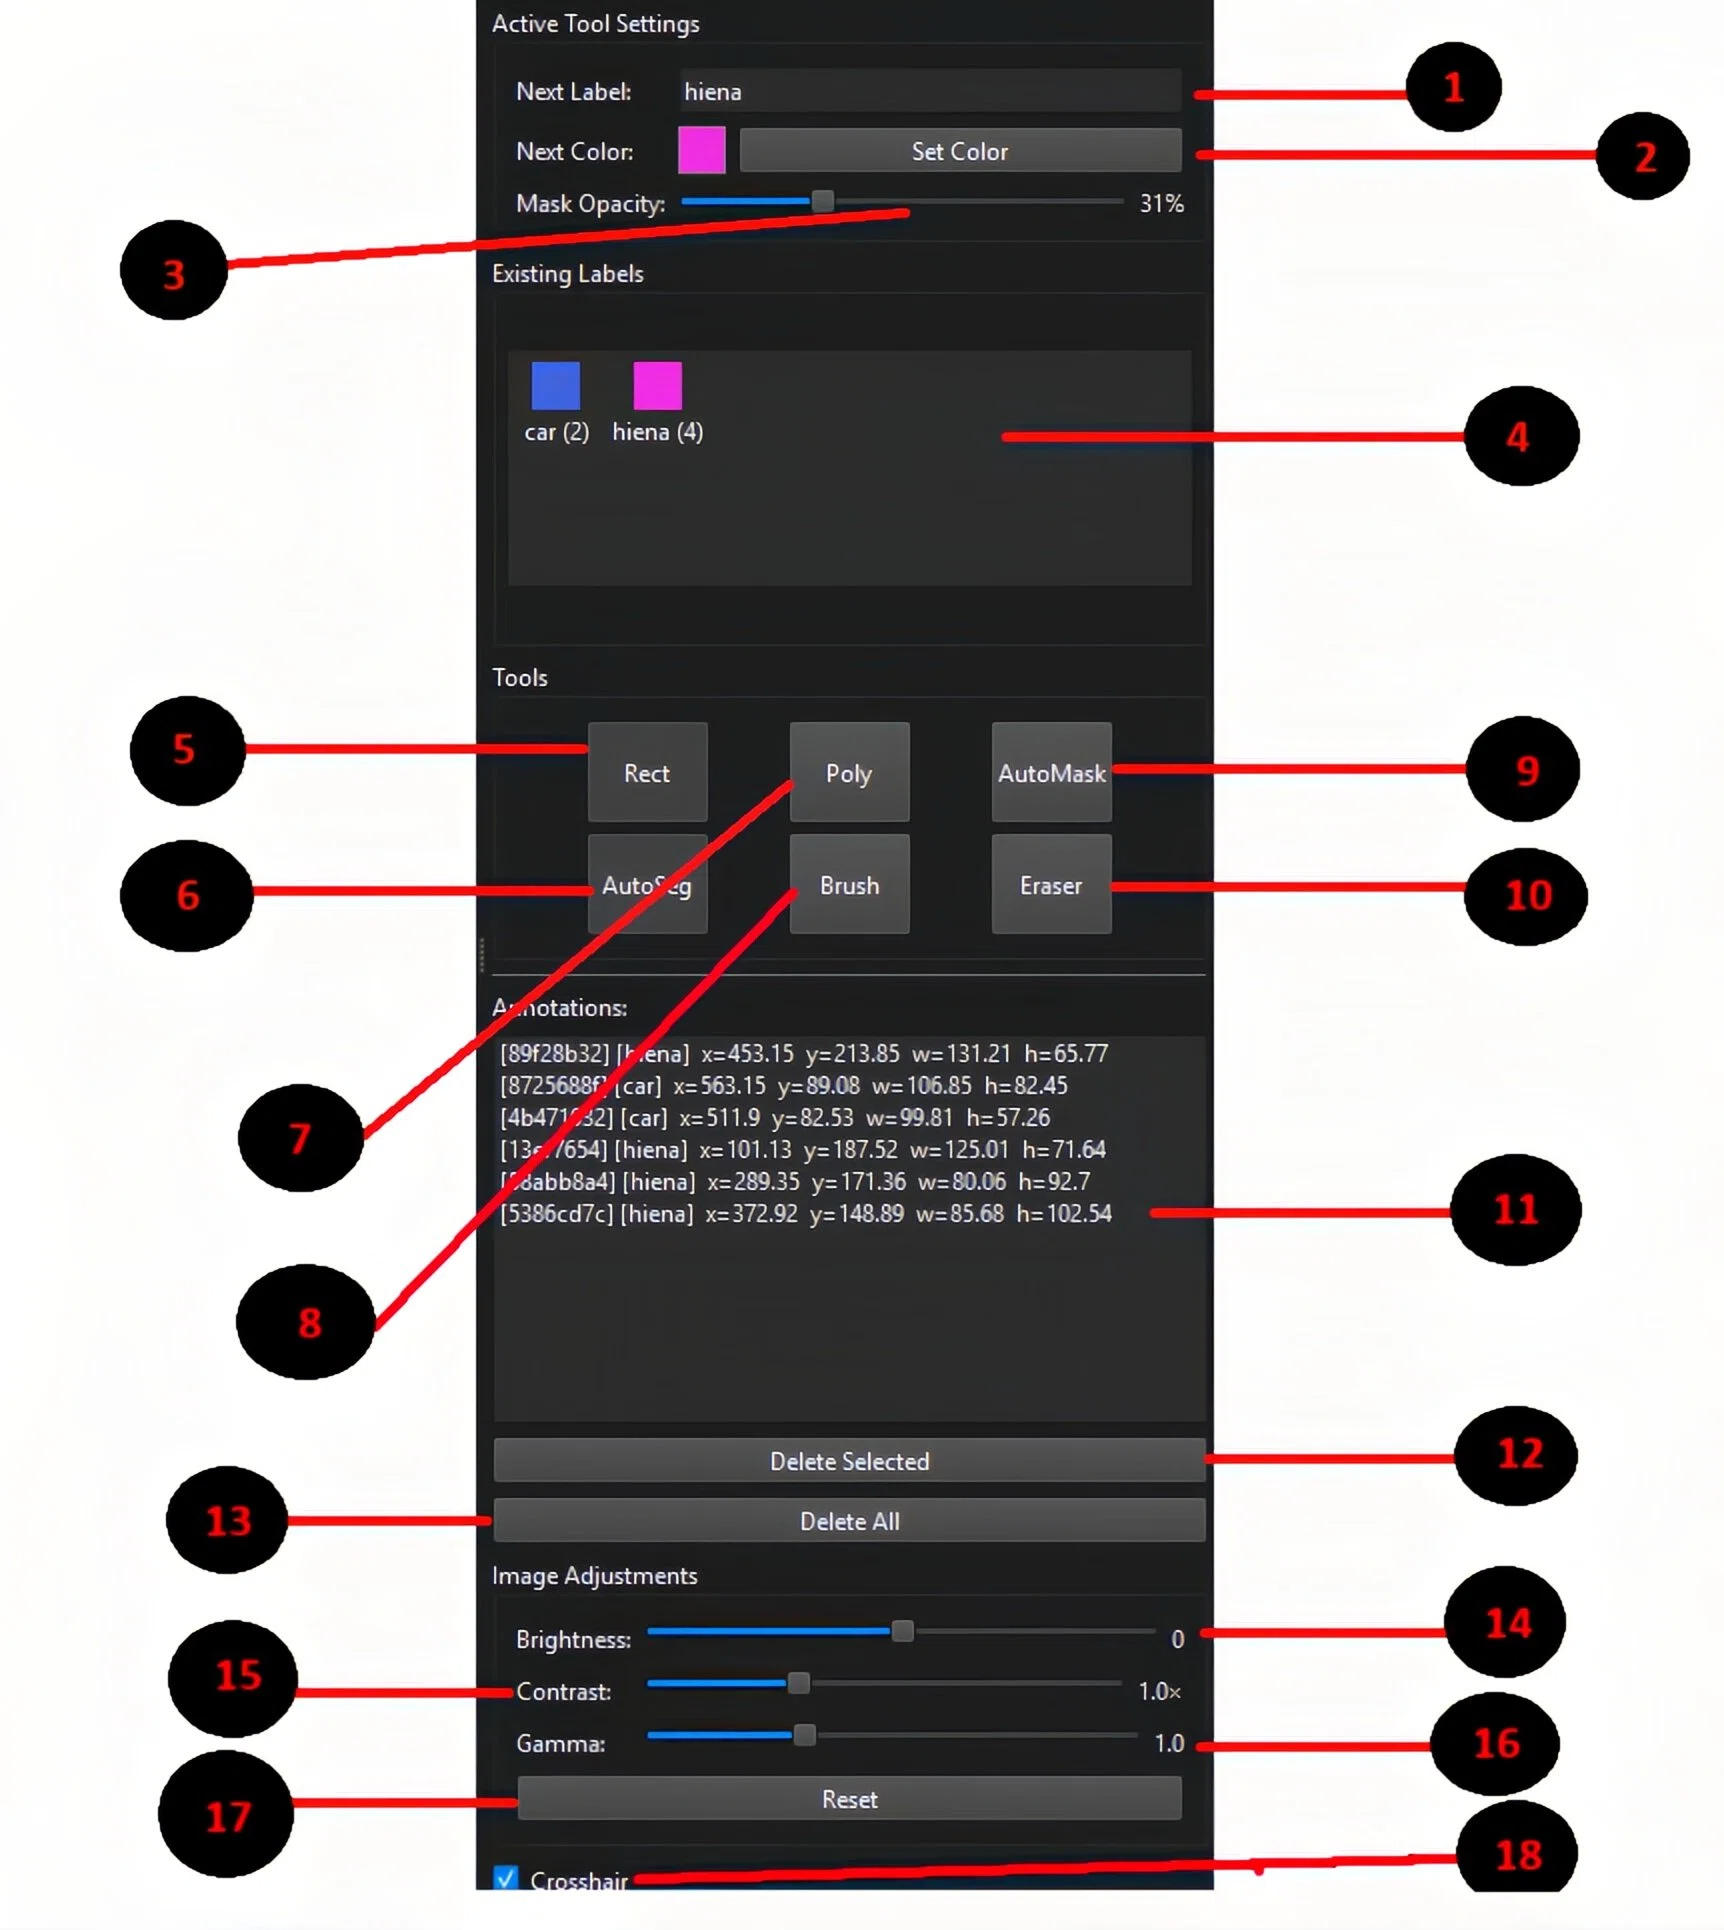
\includegraphics[width=0.46\textwidth]{figs/right_panel.png}
    \caption{Panoul de proprietăți și lista de adnotări}
    \label{fig:panou-proprietati-adnotari}
\end{figure}

Un aspect important al panourilor este că ele nu sunt simple containere vizuale. Fiecare panou deține o parte din logica de interacțiune apropiată de interfață: \texttt{LeftPanel} decide când trebuie cerută salvarea înainte de schimbarea imaginii, \texttt{ToolbarPanel} decide cum se declanșează salvarea sau exportul, iar \texttt{RightPanel} decide cum se schimbă unealta activă și cum se actualizează proprietățile unei adnotări selectate. Totuși, operațiile care afectează sistemul în ansamblu sunt propagate către \texttt{MainWindow}, canvas sau manager, păstrând o delimitare practică între UI și starea aplicației.

\subsection{Canvasul de adnotare}

Canvasul este implementat prin clasa \texttt{AnnotationCanvas}, derivată din \texttt{QGraphicsView}. Această alegere permite folosirea unui \texttt{QGraphicsScene} în care imaginea, adnotările, marker-ele temporare și elementele de feedback pot fi reprezentate ca obiecte grafice separate. Imaginea încărcată este afișată ca \texttt{QGraphicsPixmapItem}, iar adnotările sunt adăugate peste ea cu valori de \texttt{Z} mai mari, astfel încât să rămână vizibile și selectabile.

\begin{verbatim}
self._scene = QGraphicsScene(self)
self.setScene(self._scene)
self.setTransformationAnchor(
    QGraphicsView.ViewportAnchor.AnchorUnderMouse
)
\end{verbatim}

Coordonatele folosite în canvas sunt coordonate de scenă, iar scena este aliniată cu dimensiunile imaginii. Aceasta înseamnă că un punct din scenă corespunde direct unui pixel din imagine, indiferent de nivelul de zoom sau de poziția scroll-ului. Această decizie simplifică exportul și sincronizarea, deoarece adnotările pot fi salvate în coordonate ale imaginii originale, nu în coordonate dependente de interfață.

Canvasul gestionează interacțiuni specifice lucrului cu imagini: zoom cu rotița mouse-ului, pan cu butonul din mijloc sau cu \texttt{Space} și drag, desenare de dreptunghiuri, desenare de poligoane, editare de măști cu brush sau eraser și apelarea AutoMask prin click. Pentru ca fișierul \texttt{canvas.py} să nu devină greu de urmărit, evenimentele sunt extrase în \texttt{utils/canvas\_helpers/canvas\_events.py}, iar funcțiile de randare și ajustare vizuală sunt extrase în module separate. Clasa \texttt{AnnotationCanvas} rămâne astfel interfața publică a canvasului, în timp ce detaliile de mouse, tastatură și desenare sunt grupate pe fișiere tematice.

\begin{figure}[H]
    \centering
    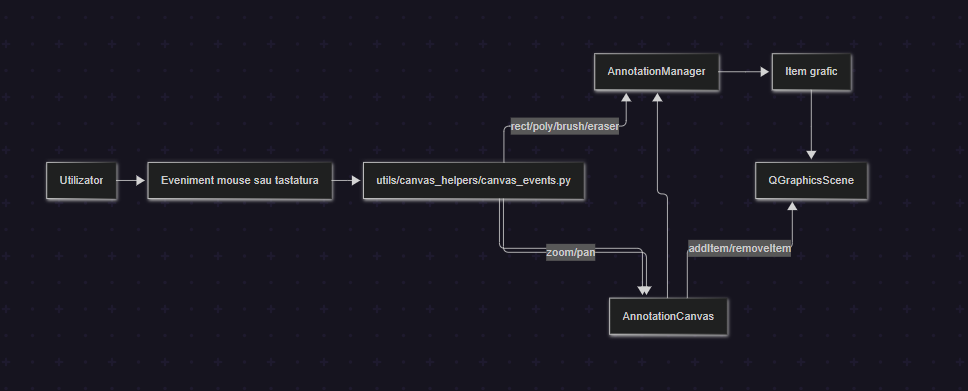
\includegraphics[width=\textwidth]{figs/Fluxul_de_evenimente_in_canvas.png}
    \caption{Fluxul de evenimente în canvas}
    \label{fig:flux-evenimente-canvas}
\end{figure}

Unealta de dreptunghi funcționează prin memorarea punctului de pornire, desenarea temporară a unui \texttt{rubber band} și transformarea dreptunghiului final într-un \texttt{BoundingBoxItem}. Unealta de poligon adaugă puncte succesive în lista internă, afișează linii temporare și finalizează conturul la click dreapta, dublu click sau tasta \texttt{Enter}. Pentru brush și eraser, canvasul caută masca selectată și trimite poziția curentă către metodele \texttt{paint\_brush()} sau \texttt{erase\_brush()} ale obiectului \texttt{MaskItem}. În cazul AutoMask, click-ul pe imagine nu creează direct o adnotare, ci emite semnalul \texttt{autoseg\_requested}, care este preluat de fereastra principală și transformat într-un apel către worker.

Canvasul conține și ajustări vizuale pentru imagine: luminozitate, contrast și gamma. Aceste ajustări nu modifică fișierul original și nu schimbă coordonatele adnotărilor. Ele sunt aplicate doar pixmapului afișat, pe baza imaginii originale păstrate în memorie. Această diferență este importantă deoarece utilizatorul poate îmbunătăți vizibilitatea unei imagini întunecate sau slabe fără să altereze datele care vor fi exportate.

\subsection{Obiectele grafice de adnotare}

Adnotările sunt gestionate de \texttt{AnnotationManager}, care funcționează ca sursă locală de adevăr pentru imaginea curentă. Managerul păstrează un dicționar de obiecte grafice indexate după identificator și emite semnale atunci când o adnotare este adăugată, ștearsă, actualizată sau când lista este golită. Aceleași semnale sunt folosite pentru actualizarea panoului drept, marcarea modificărilor nesalvate și trimiterea evenimentelor de colaborare.

\begin{verbatim}
def get_all_dicts(self) -> list[dict]:
    return [item.to_dict() for item in self._annotations.values()]
\end{verbatim}

Fragmentul arată una dintre ideile centrale ale implementării: adnotările sunt obiecte grafice, dar pot fi transformate în dicționare serializabile. Acest lucru permite folosirea aceluiași model intern atât pentru desenare pe canvas, cât și pentru salvare, export, colaborare și încărcare din fișiere.

Pentru bounding box-uri se folosește clasa \texttt{BoundingBoxItem}, derivată din \texttt{QGraphicsRectItem}. Aceasta desenează dreptunghiul, fundalul semitransparent, eticheta și mânerele de redimensionare. Atunci când un dreptunghi este selectat, utilizatorul poate modifica dimensiunea prin cele opt handle-uri. La finalul modificării geometriei, itemul notifică managerul, iar restul interfeței se actualizează prin semnale.

Pentru adnotările poligonale se folosește \texttt{PolygonItem}, derivată din \texttt{QGraphicsPolygonItem}. Aceasta reprezintă contururi definite prin puncte și are o implementare mai simplă decât dreptunghiul redimensionabil. Poligonul este potrivit pentru adnotări cu formă neregulată, dar cu un număr relativ redus de vârfuri. Ca și celelalte tipuri de item, el are etichetă, culoare, stil vizual și metodă \texttt{to\_dict()}.

Pentru măști se folosește \texttt{MaskItem}, derivată din \texttt{QGraphicsPixmapItem}. Această clasă este diferită de celelalte deoarece o mască poate conține foarte multe puncte. Pentru randare eficientă, masca este transformată într-o imagine internă, colorată cu opacitate configurabilă, iar brush-ul și eraser-ul modifică direct pixmapul asociat. Această abordare reduce costul de desenare pentru măști dense și permite utilizatorului să le editeze fluent.

\begin{figure}[H]
    \centering
    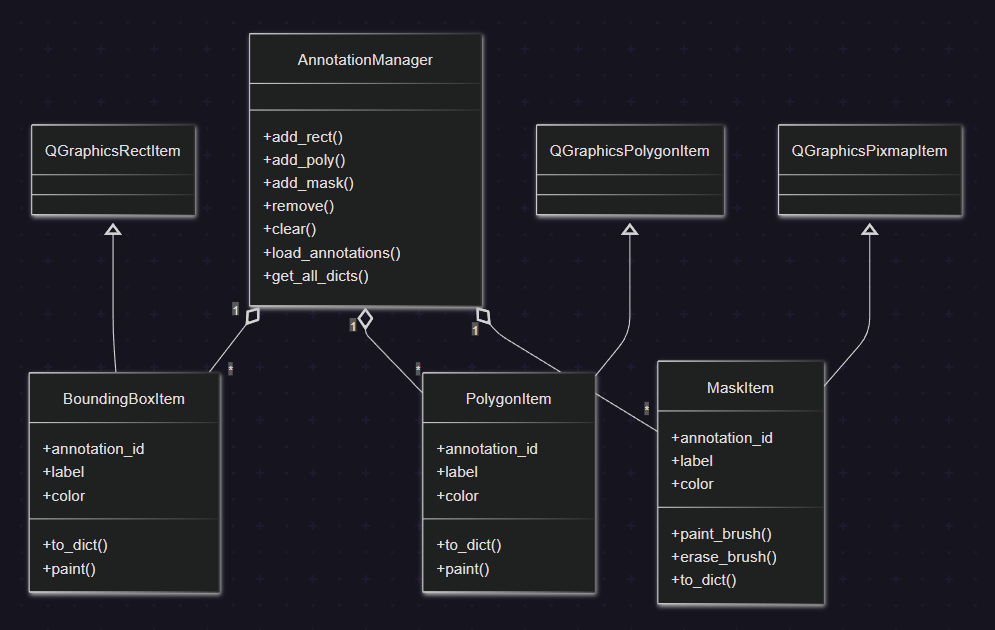
\includegraphics[width=\textwidth]{figs/Clasele_principale_pentru_adnotari.png}
    \caption{Clasele principale pentru adnotări}
    \label{fig:clase-principale-adnotari}
\end{figure}

Figura~\ref{fig:clase-principale-adnotari} poate fi transformată într-o diagramă de clase simplificată. Nu este necesară listarea tuturor metodelor, deoarece scopul este să se vadă separarea dintre manager și tipurile concrete de adnotări. Detaliile complete despre serializare și export pot fi dezvoltate în secțiunile următoare, însă introducerea acestor clase în 5.2 ajută la înțelegerea modului în care interfața și datele sunt legate.

\subsection{Integrarea AutoSeg YOLO și AutoMask în client}

Modelele de segmentare sunt integrate în client prin fluxuri de interfață, nu prin apeluri directe în canvas. Pentru AutoSeg, utilizatorul pornește operația din panoul drept prin butonul \texttt{AutoSeg}. Handler-ul \texttt{on\_autoseg\_yolo\_run()} citește setările din \texttt{QSettings}, verifică existența imaginii curente, deschide dialogul \texttt{AutoSegRunDialog} pentru etichete și moduri de ieșire, apoi pornește \texttt{AutoSegWorker}. Rezultatul poate conține \texttt{box}, \texttt{coordinates} sau \texttt{mask\_coords}, iar fiecare variantă este convertită într-un tip intern: dreptunghi, poligon sau mască.

\begin{figure}[H]
    \centering
    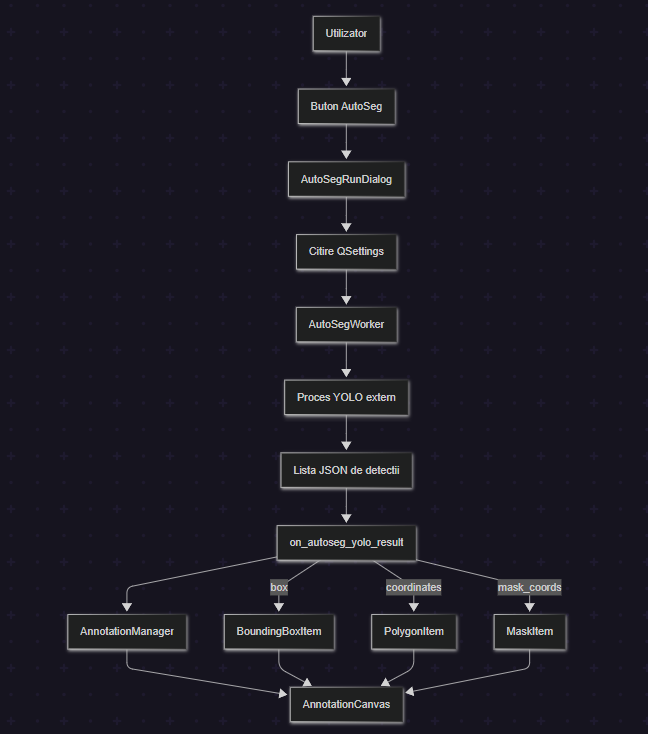
\includegraphics[width=0.78\textwidth]{figs/Fluxul_AutoSeg_YOLO_in_client.png}
    \caption{Fluxul AutoSeg YOLO în client}
    \label{fig:flux-autoseg-yolo-client}
\end{figure}

Pentru AutoMask, fluxul pornește din canvas. Utilizatorul selectează unealta AutoMask, apoi face click pe obiectul de interes. Canvasul adaugă un marker vizual temporar și emite semnalul \texttt{autoseg\_requested} cu poziția în coordonate de scenă. Handler-ul citește executabilul, timeout-ul, device-ul și argumentele suplimentare, apoi pornește \texttt{AutoMaskWorker}. Dacă modelul returnează coordonate valide, acestea sunt transformate într-o mască și adăugate pe canvas.

\begin{figure}[H]
    \centering
    
\includegraphics[width=\textwidth]{figs/Fluxul_AutoMask_pe_baza_unui_punct_selectat.png}
    \caption{Fluxul AutoMask pe baza unui punct selectat}
    \label{fig:flux-automask-punct-client}
\end{figure}

Ambele fluxuri folosesc \texttt{QProgressDialog}, astfel încât utilizatorul vede că procesarea este în curs și poate anula operația. Anularea nu se face prin închiderea brutală a aplicației sau prin blocarea firului principal, ci prin metoda \texttt{cancel()} a worker-ului, care ajunge la procesul gestionat intern. Această abordare este importantă pentru modelele AI, deoarece inferența poate dura mai mult decât o acțiune obișnuită de interfață.

Logica folosită în zona de cercetare arată că modelul concret nu este partea esențială a integrării, ci contractul de intrare și ieșire respectat de procesul extern. În \texttt{research/others/yoloe.py}, scriptul primește argumente precum \texttt{--image}, \texttt{--labels}, \texttt{--conf}, \texttt{--device} și \texttt{--mode}. După încărcarea modelului YOLOE și setarea claselor cerute, scriptul rulează predicția și scrie în \texttt{stdout} o listă JSON de detecții. Fiecare detecție poate conține eticheta, scorul de încredere, coordonatele dreptunghiului și coordonatele segmentării.

\begin{verbatim}
[
  {
    "label": "car",
    "confidence": 0.87,
    "box": [120.0, 80.0, 340.0, 250.0],
    "coordinates": [[130.0, 90.0], [330.0, 95.0], [320.0, 240.0]]
  }
]
\end{verbatim}

\texttt{AutoSegWorker} așteaptă ca rezultatul procesului să poată fi interpretat ca listă JSON. Dacă procesul întoarce un singur obiect JSON, worker-ul îl transformă într-o listă cu un singur element, dar handler-ul principal lucrează tot cu o listă de detecții. În \texttt{on\_autoseg\_yolo\_result()}, câmpul \texttt{box} este convertit într-un \texttt{BoundingBoxItem}, iar câmpul \texttt{coordinates} este convertit într-un \texttt{PolygonItem}. Există și suport pentru cheia \texttt{mask\_coords}, care poate fi transformată direct într-un \texttt{MaskItem}. Astfel, AutoSeg nu depinde strict de o anumită implementare YOLO, ci de faptul că procesul extern returnează câmpuri pe care clientul le poate transforma în adnotări.

În mod similar, \texttt{research/others/mask2former.py} implementează un flux de segmentare pe baza unui punct. Scriptul primește \texttt{--image}, \texttt{--point}, \texttt{--model} și \texttt{--device}, verifică dacă punctul se află în imagine, rulează Mask2Former și identifică segmentul pe care se află punctul selectat. Rezultatul este un obiect JSON care conține eticheta segmentului, identificatorul intern, punctul interogat, coordonatele pixelilor segmentului și un dreptunghi de încadrare.

\begin{verbatim}
{
  "label": "car",
  "id": 12,
  "point_queried": [180, 140],
  "coordinates": [[130, 90], [131, 90], [132, 91]],
  "bbox": [120, 80, 340, 250]
}
\end{verbatim}

\texttt{AutoMaskWorker} verifică în mod explicit existența cheii \texttt{coordinates}; fără aceasta, rezultatul este considerat invalid pentru client. Handler-ul \texttt{on\_autoseg\_result()} transmite datele către canvas, iar canvasul creează un \texttt{MaskItem} din coordonatele primite. Cheile suplimentare, precum \texttt{label}, \texttt{id}, \texttt{point\_queried} sau \texttt{bbox}, pot fi utile pentru diagnosticare sau extensii, dar cheia necesară pentru crearea măștii este \texttt{coordinates}.

Prin urmare, YOLOE și Mask2Former sunt exemple concrete de modele folosite în dezvoltare, însă arhitectura clientului permite înlocuirea lor cu alte executabile sau scripturi. Condiția este ca acestea să accepte parametrii transmiși de worker-e și să emită în \texttt{stdout} JSON în forma așteptată de \texttt{AnnotationEngine}. Această separare face ca aplicația să fie mai flexibilă: modelul poate evolua separat, iar interfața rămâne responsabilă doar de configurare, execuție, parsare și transformarea rezultatului în adnotări editabile.

\subsection{Worker-e și procese externe}

Pentru a păstra interfața responsivă, operațiile costisitoare nu sunt executate în firul principal al aplicației. Clientul folosește mai multe worker-e bazate pe \texttt{QThread}: \texttt{AutoSegWorker} pentru segmentarea YOLO, \texttt{AutoMaskWorker} pentru segmentarea pe punct sau pe întreaga imagine, \texttt{AuthWorker} pentru autentificare, \texttt{ChatStompWorker} pentru chat, \texttt{CollabStompWorker} pentru colaborare, \texttt{OllamaChatWorker} și \texttt{LlamaChatWorker} pentru chatbot local. Fiecare worker expune semnale de succes, eroare sau rezultat intermediar, iar UI-ul reacționează la acestea.

O parte importantă a acestei structuri este \texttt{SubprocessHandler}. El este folosit pentru executarea proceselor externe asociate modelelor AI. Comenzile sunt construite ca liste de argumente, nu ca string-uri interpretate de shell. Prin folosirea \texttt{shell=False}, aplicația reduce riscul de injecție de comenzi și controlează mai bine argumentele transmise executabilului. Handler-ul verifică existența executabilului sau a scriptului, pornește procesul, colectează \texttt{stdout} și \texttt{stderr}, aplică timeout și încearcă să extragă JSON din ieșirea procesului.

\begin{verbatim}
proc = subprocess.Popen(
    command,
    stdout=subprocess.PIPE,
    stderr=subprocess.PIPE,
    text=True,
    shell=False,
)
\end{verbatim}

Pentru anulare, \texttt{SubprocessHandler} folosește o clasă \texttt{ManagedProcess}, care învelește procesul pornit și expune metoda \texttt{kill()}. Worker-ul păstrează o referință la acest proces și îl poate opri atunci când utilizatorul apasă butonul \texttt{Cancel} din dialogul de progres. După terminare, worker-ul emite fie rezultatul parsabil, fie un mesaj de eroare care este afișat în interfață.

Aceeași idee se aplică și comunicării cu serviciile locale sau backend. Worker-ele pentru Ollama și llama.cpp trimit cereri de chat fără să blocheze fereastra de chatbot. Worker-ele STOMP gestionează bucla de recepție WebSocket în fundal, iar evenimentele primite sunt aduse în interfață prin semnale Qt. Prin această structură, aplicația poate rula simultan operații de interfață, inferență AI și comunicare în timp real fără ca utilizatorul să simtă blocaje majore.

\subsection{Ferestre auxiliare: chat, colaborare și chatbot local}

Pe lângă fereastra principală, clientul poate deschide ferestre auxiliare pentru comunicare și asistență locală. \texttt{ChatWindow} este lansată din toolbar și este responsabilă pentru chatul în timp real și funcțiile colaborative. Ea nu este implementată integral într-un singur fișier, ci folosește module separate pentru construirea UI-ului, conexiune, mesaje, setări și colaborare. Această împărțire urmează aceeași idee ca la \texttt{MainWindow}: clasa principală păstrează starea și legăturile, iar detaliile operaționale sunt mutate în fișiere tematice.

\begin{figure}[H]
    \centering
    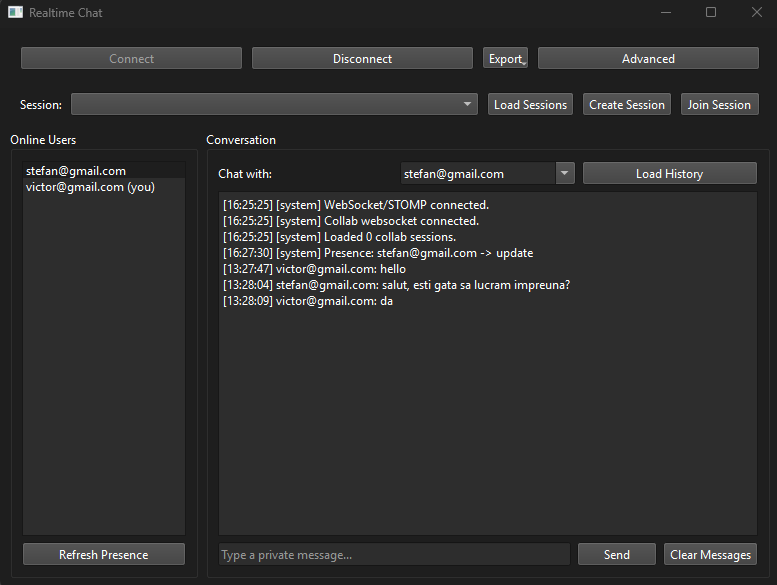
\includegraphics[width=0.9\textwidth]{figs/chat_window.png}
    \caption{Fereastra de chat și colaborare}
    \label{fig:fereastra-chat-colaborare}
\end{figure}

Pentru colaborare, \texttt{ChatWindow} se conectează la backend prin worker-e STOMP și printr-un client REST pentru operații precum listarea sesiunilor, crearea unei sesiuni sau descărcarea unei imagini partajate. Evenimentele de tip \texttt{annotation.create}, \texttt{annotation.update} și \texttt{annotation.delete} ajung înapoi în \texttt{MainWindow}, unde sunt normalizate și aplicate pe \texttt{AnnotationManager}. În sens invers, modificările locale ale adnotărilor pot fi transformate în payload-uri colaborative și trimise către sesiunea activă.

\texttt{ChatbotWindow} oferă o interfață pentru modele conversaționale locale. Utilizatorul poate alege între Ollama și llama.cpp, poate selecta sau încărca modelul dorit și poate trimite mesaje. Pentru Ollama există un worker care listează modelele disponibile și un worker care trimite cererea de chat cu streaming de tokeni. Pentru llama.cpp, fereastra permite configurarea unui fișier \texttt{GGUF}, format folosit de llama.cpp pentru stocarea modelelor, și a unor parametri precum contextul, temperatura sau numărul maxim de tokeni. Răspunsurile sunt afișate incremental, pe măsură ce worker-ul emite tokeni.

\begin{figure}[H]
    \centering
    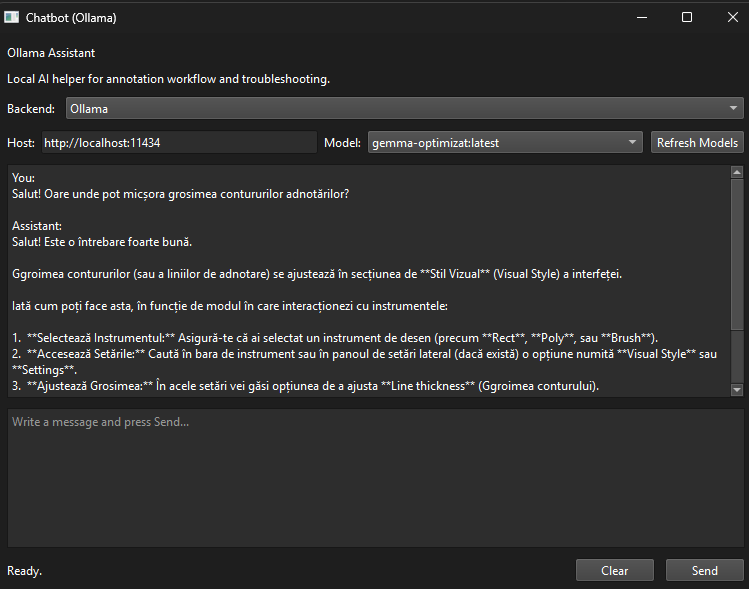
\includegraphics[width=0.9\textwidth]{figs/chatbot.png}
    \caption{Fereastra chatbot local cu Ollama sau llama.cpp}
    \label{fig:fereastra-chatbot-local}
\end{figure}

Aceste ferestre auxiliare arată că aplicația desktop nu este doar un editor de forme geometrice. Ea este punctul de intrare într-un sistem mai mare, în care utilizatorul poate cere ajutor unui LLM local, poate comunica cu alți utilizatori și poate sincroniza adnotări într-o sesiune comună. Totuși, integrarea lor este făcută astfel încât fereastra principală să rămână utilizabilă și când aceste funcții nu sunt deschise.

\subsection{Gestionarea stării locale}

O aplicație de adnotare trebuie să protejeze munca utilizatorului. În client, acest lucru este realizat printr-o stare locală de tip \texttt{\_unsaved\_changes}, care marchează dacă imaginea curentă are modificări nesalvate. Semnalele din \texttt{AnnotationManager} setează această stare atunci când se adaugă, se șterge sau se actualizează o adnotare. În anumite situații, precum încărcarea unui JSON sau aplicarea unui snapshot colaborativ, aplicația setează \texttt{\_ignore\_changes}, pentru ca operațiile programatice să nu fie interpretate ca modificări manuale ale utilizatorului.

Fluxul de schimbare a imaginii este un exemplu bun pentru această logică. Atunci când utilizatorul selectează alt fișier în \texttt{LeftPanel}, panoul verifică dacă există modificări nesalvate. Dacă nu există, emite direct cererea de încărcare. Dacă există, utilizatorul este întrebat dacă dorește să salveze înainte de schimbare. Dacă alege salvarea, panoul nu salvează singur, ci emite \texttt{save\_before\_switch\_requested}; \texttt{MainWindow} apelează salvarea din toolbar, iar apoi confirmă sau anulează schimbarea imaginii.

\begin{figure}[H]
    \centering
    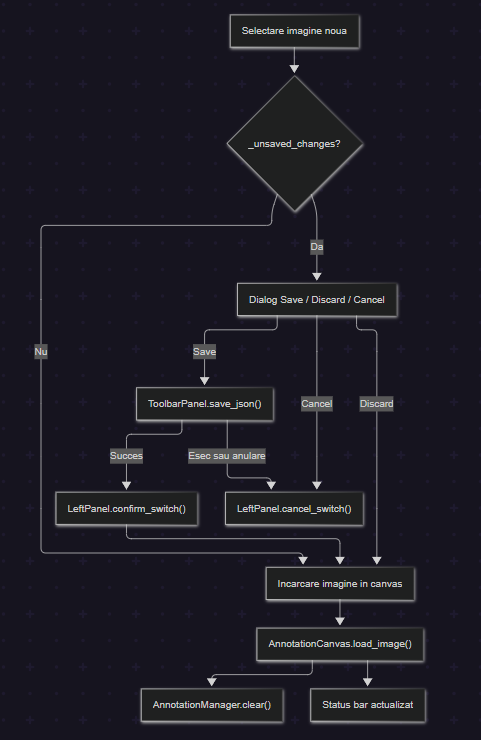
\includegraphics[width=0.62\textwidth]{figs/flux_incarcare_imagine_protectie_nesalvat.png}
    \caption{Fluxul de încărcare imagine și protecția modificărilor nesalvate}
    \label{fig:flux-incarcare-protectie-nesalvat}
\end{figure}

Fișierul \texttt{load\_process.py} grupează operațiile de încărcare a unei imagini, încărcare a adnotărilor din JSON și aplicare a setărilor vizuale. Când se importă un fișier JSON, aplicația poate încărca imaginea asociată, poate goli adnotările existente și poate reconstrui obiectele grafice prin \texttt{AnnotationManager.load\_annotations()}. Fișierul \texttt{dirty\_state.py} tratează marcarea modificărilor, resetarea stării după salvare și protecția la închiderea aplicației.

Gestionarea stării locale este importantă și pentru colaborare. Atunci când aplicația primește o actualizare de la server, flag-ul \texttt{\_applying\_remote\_collab} previne retrimiterea aceleiași modificări ca eveniment local. Pentru măști, unde editarea cu brush poate genera multe modificări într-un timp scurt, aplicația folosește un timer pentru a grupa update-urile înainte de trimitere. Astfel, clientul reduce traficul WebSocket și evită publicarea excesivă de evenimente pentru fiecare mișcare mică a mouse-ului.

Prin aceste mecanisme, clientul desktop este structurat ca o aplicație de lucru completă: are o interfață împărțită clar, un canvas interactiv, obiecte de adnotare serializabile, worker-e pentru sarcini costisitoare, ferestre auxiliare pentru colaborare și o stare locală care protejează datele utilizatorului. Această structură permite extinderea ulterioară a aplicației, de exemplu prin adăugarea unor noi tipuri de export, noi modele de segmentare sau noi instrumente de editare, fără a schimba fundamental arhitectura clientului.

\section{Autentificare și model de acces}

Partea de backend începe cu serviciul de autentificare, deoarece funcțiile de chat și colaborare au nevoie de o identitate stabilă a utilizatorului. În proiect, această responsabilitate este izolată în modulul \texttt{auth\_module}, rulat în Docker ca \texttt{auth-service}. Serviciul este o aplicație Spring Boot care expune endpoint-uri REST sub prefixul \texttt{/auth} și folosește Postgres pentru stocarea conturilor. Clientul desktop nu accesează direct baza de date, ci comunică prin cereri HTTP, iar rezultatul autentificării este folosit apoi pentru restul serviciilor.

Controllerul principal este \texttt{AuthenticationController}. Acesta definește patru operații importante: \texttt{/auth/login}, \texttt{/auth/register}, \texttt{/auth/logout} și \texttt{/auth/validate}. Primele două sunt apelate direct de aplicația desktop prin \texttt{AuthWorker}, care trimite emailul și parola într-un corp JSON și așteaptă un răspuns de tip \texttt{AuthResponse}. Endpoint-ul de validare are un rol diferit: el este folosit și de Traefik ca mecanism de \texttt{forwardAuth}, astfel încât serviciile de chat și annotation să poată fi protejate fără să implementeze fiecare aceeași logică de login.

\begin{verbatim}
POST /auth/login
POST /auth/register
POST /auth/logout
GET  /auth/validate
\end{verbatim}

La înregistrare, \texttt{UserService} verifică dacă emailul există deja, criptează parola prin \texttt{PasswordEncoder} și salvează utilizatorul în tabela gestionată de repository-ul JPA (Java Persistence API). Răspunsul nu întoarce parola, ci o variantă sigură a obiectului \texttt{User}, care conține identificatorul și emailul. Această separare este importantă deoarece aplicația desktop are nevoie doar de identitatea utilizatorului, nu de detalii interne despre credențiale.

La autentificare, \texttt{UserService.login()} folosește \texttt{AuthenticationManager} pentru verificarea parolei, iar apoi generează un token JWT prin \texttt{JWTUtils}. În implementarea curentă, token-ul are ca subiect emailul utilizatorului, include un claim \texttt{roles} și este semnat cu o cheie HMAC (Hash-based Message Authentication Code) SHA-256 (Secure Hash Algorithm 256-bit) configurată prin variabila \texttt{JWT\_SECRET}. Durata de expirare este definită în cod la 24 de ore. Structura generală a unui token JWT a fost prezentată anterior în Figura~\ref{fig:jwt-structure}; în capitolul de implementare este important mai ales modul în care token-ul circulă între componente.

După login, clientul salvează payload-ul primit local, prin \texttt{utils/auth\_store.py}. Salvarea se face în directorul de aplicație furnizat de \texttt{QStandardPaths}, într-un fișier JSON asociat sesiunii curente. În acest mod, fereastra de chat și fluxurile de colaborare pot reutiliza token-ul fără ca utilizatorul să introducă datele de autentificare la fiecare operație. Token-ul este apoi trimis în header-ul \texttt{Authorization: Bearer ...} pentru cererile REST și pentru conexiunile WebSocket/STOMP.

Endpoint-ul \texttt{/auth/validate} extrage token-ul din header, verifică forma \texttt{Bearer}, citește subiectul cu \texttt{JWTUtils.extractUsername()} și respinge token-urile expirate sau invalide. Dacă token-ul este valid, răspunsul conține header-ul \texttt{X-User-Id}. Acest header este relevant pentru serviciile aflate în spatele proxy-ului: Traefik poate valida cererea la \texttt{auth-service}, iar serviciul țintă poate primi identitatea utilizatorului fără să refacă întregul flux de autentificare.

Logout-ul este tratat stateless. Endpoint-ul \texttt{/auth/logout} extrage numele utilizatorului din token și apelează \texttt{UserService.logout()}, dar implementarea nu menține o listă de token-uri revocate. Această decizie este coerentă cu folosirea JWT în forma sa simplă: serverul nu păstrează sesiuni active pentru fiecare login, iar valabilitatea token-ului este controlată prin semnătură și timp de expirare. Pentru o variantă de producție s-ar putea adăuga o listă de revocare sau refresh token-uri, dar pentru proiectul curent fluxul este suficient pentru protejarea serviciilor colaborative.

Un detaliu important este publicarea evenimentului de înregistrare în RabbitMQ. După salvarea unui utilizator nou, \texttt{UserService} construiește un \texttt{EventMessage} cu emailul, timestamp-ul și tipul \texttt{register}, îl serializează JSON și îl publică în exchange-ul \texttt{auth.events}, cu routing key-ul \texttt{auth.user.register}. Serviciile care au nevoie să cunoască utilizatorii, cum este chatul, se pot sincroniza ascultând acest eveniment. Astfel, autentificarea rămâne sursa principală pentru conturi, iar celelalte module nu trebuie să acceseze direct baza Postgres de auth.

Din perspectiva aplicației desktop, fluxul complet este simplu. Utilizatorul deschide dialogul de cont, introduce emailul și parola, \texttt{AuthWorker} trimite cererea către endpoint-ul configurat, iar la succes payload-ul este salvat local. Ulterior, când utilizatorul deschide chatul sau colaborarea, același token este atașat la conexiunile REST și WebSocket. Astfel, autentificarea este integrată în aplicație fără să blocheze interfața și fără să amestece logica de cont cu logica de adnotare.

\section{Chat în timp real și prezență}

Serviciul de chat este separat de serviciul de annotation. Această separare există deoarece mesajele private, prezența utilizatorilor și istoricul conversațiilor au un model diferit față de sincronizarea adnotărilor. În \texttt{chat\_module}, comunicarea se face prin WebSocket peste STOMP, iar controllerul principal este \texttt{ChatController}. Clientul desktop folosește \texttt{ChatStompWorker}, un \texttt{QThread} care deschide conexiunea WebSocket, trimite frame-ul STOMP \texttt{CONNECT}, face subscribe la destinațiile relevante și procesează mesajele primite în fundal.

Endpoint-ul WebSocket al serviciului este \texttt{/ws}. În \texttt{WebSocketConfig}, aplicația configurează brokerul simplu pentru prefixele \texttt{/topic} și \texttt{/queue}, prefixul de aplicație \texttt{/app} și prefixul de user \texttt{/user}. Configurația înregistrează același endpoint \texttt{/ws} atât cu SockJS, cât și fără SockJS. În clientul desktop se folosește conexiunea WebSocket directă, dar existența variantei SockJS permite fallback pentru clienți care nu pot folosi WebSocket nativ.

\begin{verbatim}
SEND      /app/chat.send
SEND      /app/chat.history
SEND      /app/chat.presence
SUBSCRIBE /user/queue/private
SUBSCRIBE /user/queue/history
SUBSCRIBE /user/queue/presence
SUBSCRIBE /topic/presence
\end{verbatim}

Trimiterea unui mesaj privat începe în client prin \texttt{ChatStompWorker.send\_private()}. Worker-ul pune comanda într-o coadă internă, iar bucla de execuție o transformă într-un frame STOMP cu destinația \texttt{/app/chat.send}. Serverul primește mesajul în \texttt{ChatController.sendPrivateMessage()}, extrage utilizatorul curent din \texttt{Principal} și apelează \texttt{ChatService.sendPrivateMessage()}. Serviciul normalizează emailurile, verifică faptul că destinatarul există și respinge mesajele goale sau conversațiile directe cu sine.

Istoricul este păstrat în memorie, într-un \texttt{ConcurrentHashMap} care mapează cheia conversației la o coadă de mesaje. Cheia conversației este construită ordonat din cele două emailuri, astfel încât conversația dintre A și B să fie aceeași indiferent cine trimite mesajul. Pentru fiecare conversație se păstrează cel mult \texttt{MAX\_MESSAGES\_PER\_CONVERSATION}, valoare definită la 200. Când limita este depășită, mesajele cele mai vechi sunt eliminate. Această alegere reduce memoria folosită de serviciu și este potrivită pentru un backend de colaborare live, unde exportul final al datasetului nu depinde de istoricul complet de chat.

După validare, același mesaj este trimis prin \texttt{SimpMessagingTemplate} atât către expeditor, cât și către destinatar, pe coada \texttt{/queue/private}. Din perspectiva clientului, acest lucru înseamnă că fereastra de chat primește și mesajele trimise local, nu doar pe cele venite de la celălalt utilizator. Astfel, interfața poate afișa o singură sursă de evenimente și nu trebuie să aibă o ramură separată pentru mesajele proprii.

Prezența este gestionată prin \texttt{PresenceService} și \texttt{WebSocketPresenceListener}. La conectarea unei sesiuni WebSocket, utilizatorul este marcat online, iar la deconectare este marcat offline. Evenimentele de prezență sunt publicate pe \texttt{/topic/presence}, iar snapshot-ul cerut explicit de client este trimis pe \texttt{/queue/presence}. În acest mod, fereastra de chat poate afișa utilizatorii disponibili și poate actualiza starea lor fără polling HTTP repetat.

Sincronizarea utilizatorilor dintre auth și chat se face prin RabbitMQ. \texttt{UserSyncListener} ascultă coada \texttt{chat.user.register.queue}, parsează evenimentul de tip register, normalizează emailul și creează sau actualizează utilizatorul în baza H2 a modulului de chat. Această bază nu este sursa principală de autentificare, ci o copie locală necesară pentru verificarea destinatarilor și afișarea unui nume derivat din email. Prin această soluție, chatul rămâne decuplat de Postgres-ul serviciului de auth, dar poate totuși valida că un destinatar există.

Din punct de vedere funcțional, chatul este un canal de comunicare între utilizatori, nu mecanismul prin care se sincronizează adnotările. Această delimitare este importantă în documentație: mesajele private sunt tratate ca text și istoric de conversație, în timp ce colaborarea pe imagine este tratată ca stare partajată, versionată și aplicată pe canvas. Ambele folosesc WebSocket/STOMP, dar modelele de date și regulile de aplicare sunt diferite.

\section{Colaborarea pe adnotări}

Colaborarea pe adnotări este implementată în \texttt{annotation\_module}. Acest serviciu combină endpoint-uri REST pentru inițializare cu WebSocket/STOMP pentru sincronizare live. REST-ul este folosit pentru operații care au un răspuns clar și punctual, precum listarea sesiunilor, crearea unei sesiuni, obținerea unui snapshot sau încărcarea temporară a imaginii. WebSocket-ul este folosit pentru evenimente care trebuie propagate rapid către toți participanții unei sesiuni: intrarea unui utilizator, părăsirea sesiunii, disponibilitatea imaginii și modificările de adnotare.

Din exterior, prin Traefik, endpoint-urile sunt accesate sub prefixul \texttt{/annotation}. În interiorul containerului, prefixul este eliminat prin middleware-ul \texttt{annotation-strip-prefix}, iar serviciul vede rutele simple \texttt{/sessions}, \texttt{/media} și \texttt{/ws}. Această diferență explică de ce în client apar constante precum \texttt{/annotation/sessions} și \texttt{/annotation/ws}, în timp ce controller-ele Spring sunt mapate la \texttt{/sessions}, respectiv \texttt{/media}.

\begin{verbatim}
GET  /annotation/sessions
POST /annotation/sessions
GET  /annotation/sessions/{sessionId}/snapshot
POST /annotation/media/upload-temp
GET  /annotation/media/temp/{imageId}?token=...
WS   /annotation/ws
\end{verbatim}

\texttt{SessionController} gestionează sesiunile colaborative. La \texttt{GET /sessions}, serviciul întoarce lista camerelor active. La \texttt{POST /sessions}, creează o sesiune nouă, generează un cod scurt de cinci caractere și marchează utilizatorul curent ca membru online. După creare, serverul publică și un eveniment \texttt{session.created} pe \texttt{/topic/sessions}, pentru ca alți clienți conectați să poată actualiza lista de sesiuni fără refresh manual.

Snapshot-ul este mecanismul prin care un client intră într-o stare consistentă înainte de a consuma evenimente live. Când utilizatorul se alătură unei sesiuni, clientul cere \texttt{/sessions/\{sessionId\}/snapshot}. Serverul verifică sau creează apartenența utilizatorului, apoi întoarce un obiect care include identificatorii sesiunii, utilizatorii, adnotările curente, metadatele imaginii și versiunea curentă. Clientul aplică snapshot-ul local, setează ultima versiune cunoscută și apoi acceptă evenimentele noi venite pe topicul sesiunii.

\texttt{MediaController} rezolvă problema imaginii partajate. Atunci când un utilizator creează sau folosește o sesiune, imaginea activă poate fi încărcată temporar prin \texttt{/media/upload-temp}. Serverul verifică dacă fișierul este o imagine validă, îi calculează dimensiunile, dimensiunea în bytes și un checksum SHA-256, apoi salvează conținutul în \texttt{TempImageStore}. Răspunsul este un \texttt{ImageMetaDto} care conține și un \texttt{downloadUrl} cu token temporar. Ceilalți clienți pot descărca imaginea prin \texttt{/media/temp/\{imageId\}}, fără ca aceasta să devină parte din datasetul final exportat.

Evenimentele live sunt tratate de \texttt{CollaborationWsController}, prin destinația STOMP \texttt{/app/collab.event}. Clientul se abonează la \texttt{/topic/sessions} pentru lista globală de sesiuni și la \texttt{/topic/sessions/\{sessionId\}} pentru evenimentele camerei active. Fiecare eveniment este încapsulat într-un \texttt{WsEventEnvelope}, structură comună pentru tipul evenimentului, actor, sesiune, versiune și payload.

\begin{verbatim}
{
  "eventId": "...",
  "type": "annotation.update",
  "sessionId": "...",
  "projectId": "...",
  "imageId": "...",
  "cameraId": "...",
  "actorId": "...",
  "version": 12,
  "timestamp": "...",
  "payload": { }
}
\end{verbatim}

Pentru evenimentele \texttt{session.user.joined} și \texttt{session.user.left}, controllerul actualizează prezența utilizatorului în sesiune și publică rezultatul către topicul camerei. Pentru \texttt{image.available}, controllerul construiește un eveniment cu metadatele imaginii și îl trimite tuturor participanților. Pentru evenimentele de adnotare, controllerul validează apartenența utilizatorului la sesiune și apelează \texttt{CollaborationService.applyAnnotationEvent()}.

\texttt{CollaborationService} este sursa de adevăr pentru starea colaborativă a sesiunilor active. Starea este păstrată în memorie, într-un \texttt{ConcurrentHashMap} numit \texttt{sessionsById}. Fiecare sesiune conține metadatele proiectului, utilizatorii, adnotările și versiunea curentă. La \texttt{annotation.create} și \texttt{annotation.update}, payload-ul este validat și salvat în mapa de adnotări a sesiunii. La \texttt{annotation.delete}, adnotarea este eliminată după identificator. După aplicare, versiunea sesiunii este incrementată și evenimentul normalizat este publicat către clienți.

Validarea este mai strictă pentru măști, deoarece o mască fără puncte nu poate fi aplicată pe canvas. În cazul unui payload de tip \texttt{mask}, serviciul caută punctele fie în \texttt{payload.points}, fie în \texttt{payload.mask.points}, verifică existența listei și validează fiecare punct ca pereche numerică finită \texttt{[x, y]}. Această validare previne propagarea unor măști incomplete care ar putea rupe randarea pe client.

Deduplicarea este gestionată de \texttt{EventDedupStore}. Fiecare \texttt{eventId} procesat este păstrat pentru o perioadă configurabilă, implicit \texttt{PT10M}. Dacă același eveniment ajunge din nou la server, serviciul îl consideră duplicat și nu îl mai aplică. Pe client există o logică similară: \texttt{CollabStompWorker} păstrează o listă limitată de evenimente văzute, iar \texttt{chat\_window\_collab.py} păstrează ultimele versiuni primite pe sesiune. Cele două mecanisme reduc riscul de aplicare repetată a aceleiași modificări după reconectări sau retry-uri.

Prin această arhitectură, colaborarea este construită ca un flux de evenimente versionate. REST-ul aduce clientul într-o stare de pornire, iar WebSocket-ul livrează diferențele apărute după aceea. Clientul nu trebuie să descarce tot proiectul la fiecare modificare, iar serverul nu trebuie să salveze permanent datasetul final. Sesiunea live rămâne în memorie, iar exportul final rămâne responsabilitatea aplicației desktop.

\subsection{Trimiterea adnotărilor mari în mai multe pachete}

Măștile pot conține foarte multe puncte, mai ales când rezultatul vine dintr-un model de segmentare sau când utilizatorul editează zona cu brush-ul. Dacă un astfel de payload ar fi trimis într-un singur frame WebSocket, există riscul ca mesajul să fie prea mare pentru client, server sau proxy. Din acest motiv, aplicația implementează un mecanism de trimitere în mai multe pachete, denumite în cod \texttt{chunk-uri}.

Mecanismul pornește în client, în modulul de colaborare al ferestrei de chat. Funcția care decide ruta de trimitere verifică evenimentele de tip \texttt{annotation.create}, \texttt{annotation.update} și \texttt{annotation.delete}. Pentru măști create sau actualizate, evenimentul este trimis întotdeauna chunked. Pentru celelalte adnotări, chunking-ul se activează doar dacă envelope-ul serializat depășește pragul de \texttt{2 * 1024} bytes. Dimensiunea fiecărui segment base64 este \texttt{8 * 1024} caractere, iar numărul maxim de reîncercări este 2.

Pașii sunt următorii. Mai întâi, evenimentul original este serializat JSON cu \texttt{ensure\_ascii=True}. Apoi, stringul JSON este encodat base64, pentru a putea fi împărțit și reasamblat fără probleme de caractere speciale. Rezultatul base64 este tăiat în N segmente, unde N depinde de dimensiunea payload-ului:

\[
N = \left\lceil \frac{\text{lungime payload base64}}{8192} \right\rceil
\]

Fiecare segment este trimis ca un eveniment nou de tip \texttt{annotation.chunk}. Evenimentul original nu mai este trimis direct; în schimb, serverul primește toate pachetele și reconstruiește evenimentul logic inițial. Payload-ul unui pachet conține identificatorul comun al transferului, sesiunea, tipul original, indexul pachetului, numărul total, encodarea și fragmentul de date.

\begin{verbatim}
{
  "type": "annotation.chunk",
  "payload": {
    "chunkId": "uuid-transfer",
    "sessionId": "abc12",
    "originalType": "annotation.update",
    "index": 0,
    "total": 4,
    "encoding": "base64",
    "data": "eyJldmVudElkIjoiLi4u"
  }
}
\end{verbatim}

Pe server, \texttt{CollaborationWsController} detectează evenimentele de tip \texttt{annotation.chunk} și le transmite către \texttt{AnnotationChunkAssemblyService}. Serviciul parsează payload-ul în \texttt{AnnotationChunkPayloadDto} și validează câmpurile obligatorii: \texttt{chunkId}, \texttt{sessionId}, \texttt{originalType}, \texttt{index}, \texttt{total}, \texttt{encoding} și \texttt{data}. \texttt{index} trebuie să fie pozitiv sau zero, \texttt{total} trebuie să fie mai mare ca zero, iar \texttt{encoding} trebuie să fie \texttt{base64}. De asemenea, \texttt{sessionId} din payload trebuie să coincidă cu \texttt{sessionId} din envelope.

Starea temporară a transferului este păstrată într-un \texttt{ConcurrentHashMap}, indexat după \texttt{chunkId} și \texttt{sessionId}. Pentru același transfer, serverul verifică faptul că toate pachetele au aceeași sesiune, același tip original, aceeași encodare și același număr total de pachete. Serverul verifică și faptul că secvența este trimisă de același actor. Dacă un pachet duplicat are același index și aceeași valoare, este acceptat ca duplicat inofensiv; dacă are același index, dar date diferite, transferul este respins.

Există și limite de protecție. Configurația modulului definește un TTL (Time To Live) implicit de \texttt{PT45S} pentru transferurile incomplete și o limită implicită de \texttt{3000000} caractere pentru payload-ul total. Dacă un transfer nu se completează la timp, este curățat periodic. Dacă totalul de caractere depășește limita, serverul oprește reasamblarea. În plus, worker-ul STOMP de colaborare are o limită de siguranță de 2MB pentru un frame trimis direct; mesajele prea mari sunt evitate înainte de a provoca reconectări repetate.

Când toate pachetele au fost primite, serverul le concatenează în ordinea indexurilor, decodează base64, parsează JSON-ul rezultat ca \texttt{WsEventEnvelope} și verifică faptul că tipul decodat coincide cu \texttt{originalType}. Evenimentul reconstituit este apoi tratat ca un eveniment normal de adnotare: se verifică apartenența utilizatorului, se aplică modificarea în \texttt{CollaborationService}, se incrementează versiunea și se publică evenimentul final pe \texttt{/topic/sessions/\{sessionId\}}.

După aplicare, serverul trimite către client un răspuns personal pe coada de chunking. Dacă totul a reușit, tipul este \texttt{annotation.chunk.ack}; dacă pachetul este invalid sau aplicarea eșuează, tipul este \texttt{annotation.chunk.error}. Clientul ignoră evenimentele brute \texttt{annotation.chunk} primite din topic, dar tratează ack-ul și eroarea. La eroare, dacă transferul mai are încercări disponibile, clientul retrimite evenimentul original ca o nouă secvență de pachete; după două încercări eșuate, utilizatorul primește mesajul că sincronizarea a eșuat.

Acest mecanism permite colaborării să suporte atât adnotări mici, precum dreptunghiuri și poligoane, cât și măști dense, fără a schimba modelul logic de eveniment. Pentru restul sistemului, o mască actualizată rămâne tot un \texttt{annotation.update}; chunking-ul este doar stratul de transport care face posibilă livrarea sigură a payload-ului mare.

\section{Serviciile backend și infrastructura Docker}

Serviciile backend sunt pornite împreună prin \texttt{docker-compose.yml}. Compoziția definește un reverse proxy Traefik, un broker RabbitMQ, o bază Postgres pentru autentificare și cele trei servicii Spring Boot: \texttt{auth-service}, \texttt{chat-service} și \texttt{annotation-service}. Fiecare serviciu are propriul \texttt{Dockerfile}, iar configurarea sensibilă sau variabilă este transmisă prin fișierul \texttt{.env} și variabile de mediu.

\begin{table}[H]
    \centering
    \small
    \begin{tabular}{p{0.24\textwidth} p{0.18\textwidth} p{0.47\textwidth}}
        \hline
        Componentă & Port & Rol \\
        \hline
        \texttt{reverse-proxy} & \texttt{80}, \texttt{8081} & Traefik, punct unic de intrare și dashboard local. \\
        \texttt{auth-service} & \texttt{8080} & Gestionează autentificarea și rutele \texttt{/auth}. \\
        \texttt{chat-service} & \texttt{8084} & Gestionează chatul, prezența și endpoint-ul \texttt{/ws}. \\
        \texttt{annotation-service} & \texttt{8085} & Gestionează sesiunile, imaginea temporară și colaborarea pe adnotări. \\
        \texttt{rabbitmq} & \texttt{5672}, \texttt{15672} & Broker AMQP și consolă de management. \\
        \texttt{postgres-auth} & \texttt{5432} & Baza persistentă pentru utilizatorii modulului de autentificare. \\
        \hline
    \end{tabular}
    \caption{Componentele backend pornite prin Docker Compose}
    \label{tab:componente-backend-docker}
\end{table}

Traefik este punctul unic de intrare pentru backend. În \texttt{dynamic.yml}, ruta \texttt{/auth} este trimisă direct către \texttt{auth-service}, deoarece loginul și registerul trebuie să fie accesibile înainte ca utilizatorul să aibă token. Rutele \texttt{/chat}, \texttt{/notifications}, \texttt{/ws}, \texttt{/monitor} și \texttt{/annotation} trec prin middleware-ul \texttt{auth-forward}. Acest middleware apelează \texttt{http://auth-service:8080/auth/validate}; dacă token-ul este valid, cererea continuă către serviciul țintă, iar header-ul \texttt{X-User-Id} poate fi transmis mai departe.

\begin{verbatim}
/auth        -> auth-service:8080
/ws          -> chat-service:8084
/chat        -> chat-service:8084
/annotation  -> annotation-service:8085
\end{verbatim}

Pentru \texttt{/annotation}, Traefik aplică și middleware-ul \texttt{annotation-strip-prefix}. Acesta elimină prefixul \texttt{/annotation} înainte ca cererea să ajungă la serviciul Spring Boot. De aceea, clientul folosește ruta publică \texttt{/annotation/sessions}, dar \texttt{SessionController} este mapat intern la \texttt{/sessions}. Această soluție permite păstrarea unor rute publice clare, fără ca serviciul intern să fie obligat să cunoască prefixul de proxy.

RabbitMQ este folosit pentru evenimente între servicii, nu pentru mesajele live de colaborare din canvas. În implementarea curentă, cel mai clar exemplu este evenimentul de înregistrare a utilizatorului. \texttt{auth-service} publică evenimentul în exchange-ul \texttt{auth.events}, iar \texttt{chat-service} îl consumă prin coada \texttt{chat.user.register.queue}. \texttt{annotation-service} are de asemenea configurare RabbitMQ, ceea ce păstrează posibilitatea extinderii mecanismului de sincronizare între servicii, chiar dacă starea colaborativă live este gestionată prin WebSocket.

Postgres este folosit doar pentru zona de autentificare. În \texttt{docker-compose.yml}, serviciul \texttt{postgres-auth} pornește imaginea \texttt{postgres:15}, creează baza de auth, folosește un volum persistent și rulează scripturi de inițializare din directorul modulului de autentificare. \texttt{auth-service} depinde de healthcheck-ul Postgres și primește URL-ul JDBC (Java Database Connectivity) prin variabile de mediu. Această dependență face ca serviciul de auth să pornească numai după ce baza poate accepta conexiuni.

Serviciile \texttt{chat-service} și \texttt{annotation-service} sunt expuse doar în rețeaua Docker prin \texttt{expose}, nu prin porturi publice directe. Clientul desktop le accesează prin Traefik, folosind \texttt{localhost} ca bază publică. Această alegere simplifică configurarea clientului: în loc ca aplicația să cunoască trei porturi diferite, ea poate folosi același host, iar proxy-ul decide serviciul țintă în funcție de prefix.

Din punct de vedere operațional, Docker Compose oferă o structură reproductibilă pentru backend. Se pornesc serviciile, brokerul și baza de date în aceeași rețea, cu aceleași nume DNS (Domain Name System) interne. Spring Boot primește configurația prin variabile de mediu, iar codul clientului poate rămâne orientat spre endpoint-uri stabile. Această structură nu transformă aplicația într-un sistem distribuit complex, dar separă clar responsabilitățile și permite testarea independentă a fiecărui serviciu.

\section{Persistența și structura datelor}

Persistența datelor este împărțită în funcție de natura fiecărui tip de informație. Nu toate datele au aceeași durată de viață. Conturile utilizatorilor trebuie să supraviețuiască restarturilor, conversațiile sunt utile în timpul rulării serviciului de chat, sesiunile colaborative sunt stări live, iar datasetul final este produs local prin export din clientul desktop. Această împărțire evită salvarea inutilă a unor date temporare și păstrează mai clar rolul fiecărei componente.

Pentru autentificare se folosește Postgres. Aici sunt salvate conturile, emailurile și parolele criptate. Această informație este persistentă și are nevoie de consistență între porniri, deoarece utilizatorul trebuie să poată reveni în aplicație cu același cont. Volumul Docker \texttt{postgres-auth-data} păstrează datele bazei între rulări, iar JPA gestionează entitățile modulului de auth.

Pentru chat, serviciul folosește H2 în memorie pentru repository-ul de utilizatori sincronizați și o structură \texttt{ConcurrentHashMap} pentru istoricul conversațiilor. Mesajele private nu sunt salvate în Postgres; ele rămân în memoria serviciului și sunt limitate la ultimele 200 de mesaje per conversație. Această alegere este potrivită pentru prototipul colaborativ, deoarece chatul este un instrument de coordonare în timpul lucrului, nu arhiva principală a proiectului.

Pentru colaborare, \texttt{annotation-service} este explicit configurat ca modul in-memory. În \texttt{application.properties}, auto-configurările JDBC și JPA sunt excluse, iar starea este păstrată în obiecte Java: \texttt{sessionsById}, adnotările pe sesiune, utilizatorii prezenți, metadatele și conținutul temporar al imaginilor, plus evenimentele procesate pentru deduplicare. Sesiunile goale și inactive sunt curățate după un TTL implicit de cinci minute, imaginile temporare au TTL de patru ore, iar evenimentele procesate sunt păstrate pentru deduplicare timp de zece minute.

Această alegere are un compromis clar. Pe de o parte, colaborarea live este rapidă și ușor de urmărit în cod, deoarece serverul nu trebuie să scrie fiecare mișcare într-o bază de date. Pe de altă parte, o repornire a \texttt{annotation-service} pierde sesiunile active. În contextul proiectului, acest compromis este acceptabil deoarece artefactul final nu este sesiunea live, ci exportul local realizat de client: JSON intern, COCO, YOLO sau imagine cu măști. Serverul ajută utilizatorii să lucreze împreună, dar nu înlocuiește mecanismul de export al aplicației desktop.

\begin{table}[H]
    \centering
    \small
    \begin{tabular}{p{0.30\textwidth} p{0.58\textwidth}}
        \hline
        Zonă de date & Mecanism folosit \\
        \hline
        Conturi utilizatori & Postgres, prin \texttt{auth-service}. \\
        Utilizatori disponibili în chat & H2 în memorie, populat din evenimente RabbitMQ. \\
        Istoric conversații & Memorie, maximum 200 mesaje per conversație. \\
        Sesiuni colaborative & Memorie, cu versiuni, utilizatori și adnotări pe sesiune. \\
        Imagini partajate temporar & Memorie, prin \texttt{TempImageStore}, cu token și TTL. \\
        Dataset final & Fișiere locale exportate de \texttt{AnnotationEngine}. \\
        \hline
    \end{tabular}
    \caption{Persistența datelor pe componente}
    \label{tab:persistenta-date-backend}
\end{table}

Separarea persistenței ajută și la explicarea limitelor sistemului. Dacă un utilizator se deloghează și revine, contul său rămâne în Postgres. Dacă serviciul de chat repornește, istoricul volatil se pierde, dar utilizatorii se pot resincroniza prin evenimentele de register și prin autentificare. Dacă o sesiune colaborativă este pierdută, adnotările trebuie recuperate din fișierele locale sau din exporturile realizate de client. Astfel, sistemul este proiectat ca un instrument de lucru și colaborare, nu ca o platformă completă de versionare permanentă a dataseturilor.

\section{Rulare și integrarea componentelor}

Pentru rularea sistemului complet sunt necesare două zone pornite separat: zona server din \texttt{ColaborativeServer} și clientul desktop din \texttt{AnnotationEngine}. Serviciile server se pornesc prin Docker Compose, ceea ce aduce în aceeași rețea Traefik, RabbitMQ, Postgres și cele trei servicii Spring Boot. Clientul desktop se rulează local și folosește endpoint-urile configurate în \texttt{QSettings} pentru autentificare, chat și colaborare.

Fluxul complet începe de obicei cu înregistrarea sau autentificarea utilizatorului. Clientul trimite cererea către ruta publică de login sau register, iar după autentificare token-ul este salvat local și devine baza pentru celelalte conexiuni. Când utilizatorul deschide fereastra de chat, worker-ul STOMP se conectează la endpoint-ul WebSocket de chat. Când utilizatorul folosește colaborarea pe adnotări, clientul REST accesează sesiunile din \texttt{/annotation/sessions}, iar worker-ul colaborativ se conectează la \texttt{/annotation/ws}.

Într-un scenariu colaborativ tipic, primul utilizator creează o sesiune, iar clientul trimite către backend identificatori pentru proiect, imagine și cameră. Dacă există o imagine activă în aplicație, ea poate fi încărcată temporar prin \texttt{/annotation/media/upload-temp}. Serverul publică apoi \texttt{image.available}, iar alți clienți pot descărca imaginea prin URL-ul temporar. După alăturare, fiecare client cere snapshot-ul sesiunii, aplică starea locală și începe să primească evenimente live.

Atunci când un utilizator creează, modifică sau șterge o adnotare, \texttt{MainWindow} transformă schimbarea locală într-un payload colaborativ. Acest payload ajunge în \texttt{ChatWindow}, care îl trimite prin \texttt{CollabStompWorker}. Pentru evenimente mici, trimiterea este directă. Pentru măști și payload-uri mari, se activează mecanismul de trimitere în N pachete. Serverul aplică evenimentul, îl versionază și îl publică înapoi către toți clienții din sesiune. Clienții care primesc evenimentul îl aplică pe \texttt{AnnotationManager}, dar folosesc flag-ul \texttt{\_applying\_remote\_collab} pentru a nu retrimite aceeași modificare.

\begin{figure}[H]
    \centering
    \small
    \setlength{\fboxsep}{5pt}
    \begin{tabular}{c}
        \fbox{\parbox{0.86\textwidth}{\centering
        \textbf{1. Autentificare:} utilizatorul face login/register, iar \texttt{auth-service} emite tokenul JWT salvat de client.}} \\
        $\downarrow$ \\
        \fbox{\parbox{0.86\textwidth}{\centering
        \textbf{2. Inițializare colaborare:} clientul cere lista de sesiuni și snapshot-ul prin endpoint-urile REST ale serviciului de annotation.}} \\
        $\downarrow$ \\
        \fbox{\parbox{0.86\textwidth}{\centering
        \textbf{3. Cameră de lucru:} \texttt{SessionController} creează sau identifică sesiunea, iar imaginea activă poate fi încărcată temporar.}} \\
        $\downarrow$ \\
        \fbox{\parbox{0.86\textwidth}{\centering
        \textbf{4. Conexiune live:} worker-ul colaborativ se abonează la topicul sesiunii și primește evenimente WebSocket/STOMP.}} \\
        $\downarrow$ \\
        \fbox{\parbox{0.86\textwidth}{\centering
        \textbf{5. Editare adnotări:} \texttt{MainWindow} construiește payload-ul, iar serverul aplică evenimentul și incrementează versiunea.}} \\
        $\downarrow$ \\
        \fbox{\parbox{0.86\textwidth}{\centering
        \textbf{6. Payload mare:} pentru măști sau date voluminoase, evenimentul este împărțit în N pachete și reasamblat pe server.}} \\
        $\downarrow$ \\
        \fbox{\parbox{0.86\textwidth}{\centering
        \textbf{7. Sincronizare:} versiunea nouă este publicată pe topicul sesiunii, iar ceilalți clienți aplică modificarea în \texttt{AnnotationManager}.}}
    \end{tabular}
    \caption{Fluxul operațional al colaborării dintre utilizator, clientul desktop și backend}
    \label{fig:flux-operational-colaborare}
\end{figure}

Modelele AI și chatbotul local se configurează separat de backend-ul Docker. AutoSeg și AutoMask pot fi executabile sau scripturi externe, iar căile lor sunt păstrate în \texttt{QSettings}. Ollama trebuie să ruleze local dacă utilizatorul alege backend-ul Ollama pentru chatbot, iar llama.cpp folosește un fișier local \texttt{GGUF}. Această separare este intenționată: backend-ul gestionează identitate și colaborare, în timp ce modelele AI sunt resurse locale controlate de client.

Prin această organizare, aplicația poate fi folosită gradual. Pentru adnotare individuală și export, utilizatorul are nevoie doar de clientul desktop și de fișierele locale. Pentru autentificare, chat și colaborare, se pornește backend-ul Docker. Pentru segmentare automată și chatbot, se configurează executabilele sau serviciile locale corespunzătoare. Sistemul nu obligă toate componentele să fie active pentru fiecare scenariu, dar le poate lega într-un flux complet atunci când utilizatorul lucrează colaborativ pe aceeași imagine.
\setlength{\parskip}{0pt}

